\documentclass[12pt]{article}

% Use special characters directly in text
\usepackage[utf8]{inputenc}
\DeclareUnicodeCharacter{2010}{-}% support older LaTeX versions
\usepackage[T1]{fontenc}
\usepackage{array}
\usepackage{tabularx}
\usepackage[margin=25mm]{geometry}
\usepackage{booktabs}
\usepackage{todonotes}
\usepackage{amsmath}
%\usepackage{hyperref}
\newcommand{\ra}[1]{\renewcommand{\arraystretch}{#1}}
% Users of the {thebibliography} environment or BibTeX should use the
% scicite.sty package, downloadable from *Science* at
% http://www.sciencemag.org/authors/preparing-manuscripts-using-latex 
% This package should properly format in-text
% reference calls and reference-list numbers.
\usepackage[export]{adjustbox}
%\usepackage[
%		style=numeric,
%		backend=biber,
%		sorting=none,
%		defernumbers=true,
%		url=false,
%		isbn=false,
%		uniquename=true]{biblatex}
%\usepackage[sorting=none,defernumbers=true]{biblatex}

\usepackage[sortcites,sorting=none,url=false,isbn=false,backend=biber,uniquename=true, defernumbers]{biblatex}



\bibliography{./References/bibliography}
% Package for line numbers
\usepackage{lineno}


% Graphics preamble
\usepackage{graphicx}
\usepackage{float}
\usepackage[font={footnotesize}]{caption} % Exclude automatic numbering of figures 
\usepackage{textcomp}

\usepackage{times}

% The preamble here sets up a lot of new/revised commands and
% environments.  It's annoying, but please do *not* try to strip these
% out into a separate .sty file (which could lead to the loss of some
% information when we convert the file to other formats).  Instead, keep
% them in the preamble of your main LaTeX source file.

% Define folder for graphics
\graphicspath{{./Plots/}}

% The following parameters seem to provide a reasonable page setup.

\topmargin 0.0cm
\oddsidemargin 0.2cm
\textwidth 16cm 
\textheight 21cm
\footskip 1.0cm

\setlength{\parindent}{0em}
\setlength{\parskip}{1em}

% This is the original, well working setup
%\topmargin 0.0cm
%\oddsidemargin 0.2cm
%\textwidth 16cm 
%\textheight 21cm
%\footskip 1.0cm

%The next command sets up an environment for the abstract to your paper.

\newenvironment{sciabstract}{%
\begin{quote} \bf}
{\end{quote}}



% Include your paper's title here
%\title{Differences in future Greenland melt controlled by cloud microphysics and circulation}


\title{The contribution of blowing snow to cloud properties and the atmospheric radiative budget over Antarctica}
%\title{Doubling of future Greenland Ice Sheet surface melt revealed by the new CMIP6 high-emission scenario}
%\title{Cloud microphysics and circulation anomalies control future Greenland Ice Sheet melt} 


% Place the author information here.  Please hand-code the contact
% information and notecalls; do *not* use \footnote commands.  Let the
% author contact information appear immediately below the author names
% as shown.  We would also prefer that you don't change the type-size
% settings shown here.

\author
{Stefan Hofer,$^{1\ast}$ Charles Amory,$^{2}$ Christoph Kittel,$^{2}$ Tim Carlsen$^{1}$ and Trude Storelvmo$^{1}$ \\
\\
\normalsize{$^{1}$Department of Geosciences, University of Oslo, Oslo, Norway}\\
\normalsize{$^{2}$Laboratory of Climatology, Department of Geography, University of Liège, Belgium}\\
\\
\normalsize{$^\ast$Corresponding author: Stefan Hofer, stefan.hofer@geo.uio.no}
}

% Include the date command, but leave its argument blank.

\date{}



%%%%%%%%%%%%%%%%% END OF PREAMBLE %%%%%%%%%%%%%%%%



\begin{document} 
%\begin{refsection}
% Double-space the manuscript.

\baselineskip24pt

% Make the title.

\maketitle 
%BibTeX users: After compilation, comment out the following two lines and paste in
% the generated .bbl file. 



% Place your abstract within the special {sciabstract} environment.

%\begin{sciabstract}
%  This document presents a number of hints about how to set up your
%  {\it Science\/} paper in \LaTeX\ .  We provide a template file,
%  \texttt{scifile.tex}, that you can use to set up the \LaTeX\ source
%  for your article.  An example of the style is the special
%  \texttt{\{sciabstract\}} environment used to set up the abstract you
%  see here.
%\end{sciabstract}



% In setting up this template for *Science* papers, we've used both
% the \section* command and the \paragraph* command for topical
% divisions.  Which you use will of course depend on the type of paper
% you're writing.  Review Articles tend to have displayed headings, for
% which \section* is more appropriate; Research Articles, when they have
% formal topical divisions at all, tend to signal them with bold text
% that runs into the paragraph, for which \paragraph* is the right
% choice.  Either way, use the asterisk (*) modifier, as shown, to
% suppress numbering.
\newpage
\linenumbers

\textbf{Antarctica and its surroundings are one of the main areas for biases in climate models, mostly due to uncertainties in the representation of clouds. Over the Antarctic Ice Sheet, temperature inversions and strong temperature gradients between the cold interior and the edges lead to strong katabatic downslope winds, transporting snow and moisture from the interior towards the peripheral regions at the southern edge of the Southern Ocean’s storm track. These blowing snow layers are usually 100-200 m thick, but can reach a thickness of more than 500 m and can be advected offshore from Antarctica over open ocean waters (Scarchili et al., 2010; Palm et al., 2017). However, the impacts of moisture and wind-induced snow mass transport (i.e. ice nucleating particles) on cloud structure and development over Antarctica has not been thoroughly investigated and most state-of-the-art climate models do not account for its presence. Here, we use a regional climate model with a newly developed fully active blowing snow scheme and satellite data, to show that accounting for drifting snow notably alters the spatial distribution, vertical structure and radiative contribution of clouds over Antarctica and its periphery. Additionally, our results indicate that the advection of blowing snow and air with a higher humidity content over the Southern Ocean also impacts clouds and their microphysics in areas outside of Antarctica. While our study area is limited to 60S, our results highlight the need to study the impact of missing blowing snow processes on the future evolution of clouds not just over Antarctica, but potentially also over the Southern Ocean, an area with significant uncertainties in future climate projections.}

%OLD ABSTRACT
% Here, we show that the total GrIS melt during the 21st century almost doubles when using CMIP6 forcing compared to the previous CMIP5 model ensemble, despite an equal global radiative forcing of +8.5 W/m\textsuperscript{2} in 2100 in both RCP8.5 and SSP58.5 scenarios. The total GrIS sea level rise contribution from surface melt in our high-resolution (15 km) projections is 17.8 cm in SSP58.5, 7.9 cm more than in our RCP8.5 simulations, despite the same radiative forcing. We identify a +1.7\textdegree C greater Arctic amplification in the CMIP6 ensemble as the main driver behind the presented doubling of future GrIS sea level rise contribution.

%
\section*{Introduction} 

\textbf{First paragraph:} Main facts about Antarctica and clouds there
Radiative effects, influence on surface temperature (SEB). a bit about melt (even in winter; see Kuipers-Munneke 2014).

Antarctica is the largest body of ice on the planet and it contains the coldest places on Earth.  It contains ice mass equivalent to roughly \textbf{XX m} of global sea level rise, roughly 10 times more than the Greenland Ice Sheet (\textbf{cite XX}). The interior plateau of the Antarctica reaches up to elevations of \textbf{XX m}, and is marked by very cold and dry conditions (\textbf{cite XX}). However, there are marked differences in the present climatic conditions between East and West Antarctica, and especially between the edges and the inner plateau. While West Antarctica, and especially the northwards reaching mountainous Antarctic peninsula receive ample precipitation and are rather cloudy, weather systems never reach the interior of Antarctica, where most of the precipitation falls as diamond dust under extremely cold  "clear" sky conditions (cite XX). 

Due to strong radiative cooling in the interior plateau, strong and perpetual katabatic winds emerge, redistributing snow mass from the interior towards the edges and ice shelves, where the up to \textbf{XX m} high plateau slopes steeply towards sea level (\textbf{CITE XX}). 

\textbf{Second paragraph:} describing BS as near-surface clouds + source of moisture and condensation nuclei for additional cloud formation in the lower atmosphere

\textbf{Third paragraph:} What are the open questions? 
i) Does BS lead to improved representation of cloud properties in the model and ii) how does it affect the representation of clouds?

Clouds are known to notably affect the present and future climates of polar ice sheets \cite{Hofer2017, Hofer2019, VanTricht2016, Izeboud2020, Hahn2019}. Clouds have the ability to amend incoming shortwave and longwave fluxes, depending on the cloud phase, height and particle size distribution, impacting the rate of surface melt and snowpack warming. Blowing snow, while not accounted for in most global and regional climate models, can change the vertical structure and radiative impact of clouds, most notably because blowing snow sublimation changes the atmospheric humidity and temperature distribution (cite Louis 2020). Blowing snow particles can also act as ice nucleating particles for cloud formation, which also impacts the longevity, structure and cloud-phase distribution within pre-existing clouds. Additionally, optically thick blowing snow layers can act as a cloud themselves, increasing the atmospheric longwave emissivity and shortwave transparency of the atmosphere. However, so far very little is known about how clouds are influenced by blowing snow processes in climate models, and how accounting for blowing snow over the current climate influences key polar cloud-, and therefore climate processes.

\textbf{Fourth paragraph:} How are we planning to address the questions? 
Two sets of simulations + satellite products

Here, we use two regional climate model simulations spanning the period of 1979-2019, one with a dynamic representation of blowing snow and one without, to assess the impact of accounting for blowing snow on Antarctic clouds and radiative fluxes. We compare our two simulations to satellite products of cloud cover and the ERA5 reanalysis product, to show whether accounting for drifting snow only amends or also improves the representation of polar clouds. However, due to the remote location and complications of detecting cloud structure and microphysics from satellites over highly reflective surfaces, we don’t expect to comprehensively address whether blowing snow improves cloud representation over Antarctica. Nevertheless, our results deliver a clear indication that accounting for blowing snow over polar ice sheets changes the 3D-structure of clouds, their phase and ultimately their contribution to the surface energy budget. In conclusion, not accounting for drifting snow in future projections of the Antarctica climate and sea level rise contribution might significantly bias the drawn conclusions.  

\section*{Results}

%For a comparison between the regional climate response of Greenland in the high-emission scenario in CMIP5 and CMIP6, we forced the regional climate model MAR with 6 general circulation models (GCMs) from the CMIP5 model suite \cite{Taylor2012,Moss2010} and 5 GCMs from the CMIP6 project \cite{Eyring2016,ONeill2016}. From the CMIP5 project we chose the Representative Concentration Pathway 8.5 scenario, while we chose the SSP58.5 scenario for the CMIP6 models. Both of these high-emission scenarios correspond to a surface energy budget (SEB) forcing due to greenhouse gas emissions of 8.5 W/m\textsuperscript{2} in 2100 \cite{Moss2010,Taylor2012,Eyring2016,ONeill2016}.

\textbf{Influence of blowing snow on the vertical atmospheric structure}

Explicitly modelling blowing in snow in MAR leads to a notable change in the atmospheric structure of the lowermost 100s of meters above ground (Fig.\ref{fig:Test} A-C). Over the flat interior of the Antarctic Ice Sheet, the first few 100 m show a strong decrease in atmospheric temperature, with a mean 0-500 m difference of \textbf{XX $\pm$ XX \textdegree C} in elevations greater than 2000 m above mean sea level (Fig.\ref{fig:Test} A). This cooling of the near-surface atmosphere in our MAR blowing snow simulations, when compared to MAR without blowing snow, is most likely due to the efficient sublimation of airborne blowing snow particles due to the dry (and cold) surroundings over the interior Antarctic plateau. Conversely, over the steep slopes and the flat, low-lying ice shelves surrounding the grounded ice, this decrease in temperature in the blowing snow simulations is less notable. The mean 0-500 m above surface difference lies at \textbf{XX pm XX \textdegree C}. The contrasting picture between the flat interior and the steeper and lower margins of Antarctica is likely due to two effects: 1) Due to the on average lower relative humidity and the greater water vapour gradients, the airborne blowing snow particles are more readily sublimated in the drier interior plateau than over the margins. This change of phase from solid to gaseous requires energy from the surrounding air to break up the bonds between the H$_2$O molecules (\textbf{CITE CC}), leading to a drop in temperature. 2) Due to strong adiabatic mixing and turbulence in areas where the gravitational pull accelerates the katabatic winds down steep terrain, the snow particles are not confined to the very stable boundary layer anymore. Therefore, the sublimational cooling is less concentrated and subsequently also lower in magnitude over the margins of Antarctica and the ice shelves.

\begin{figure}[H]
	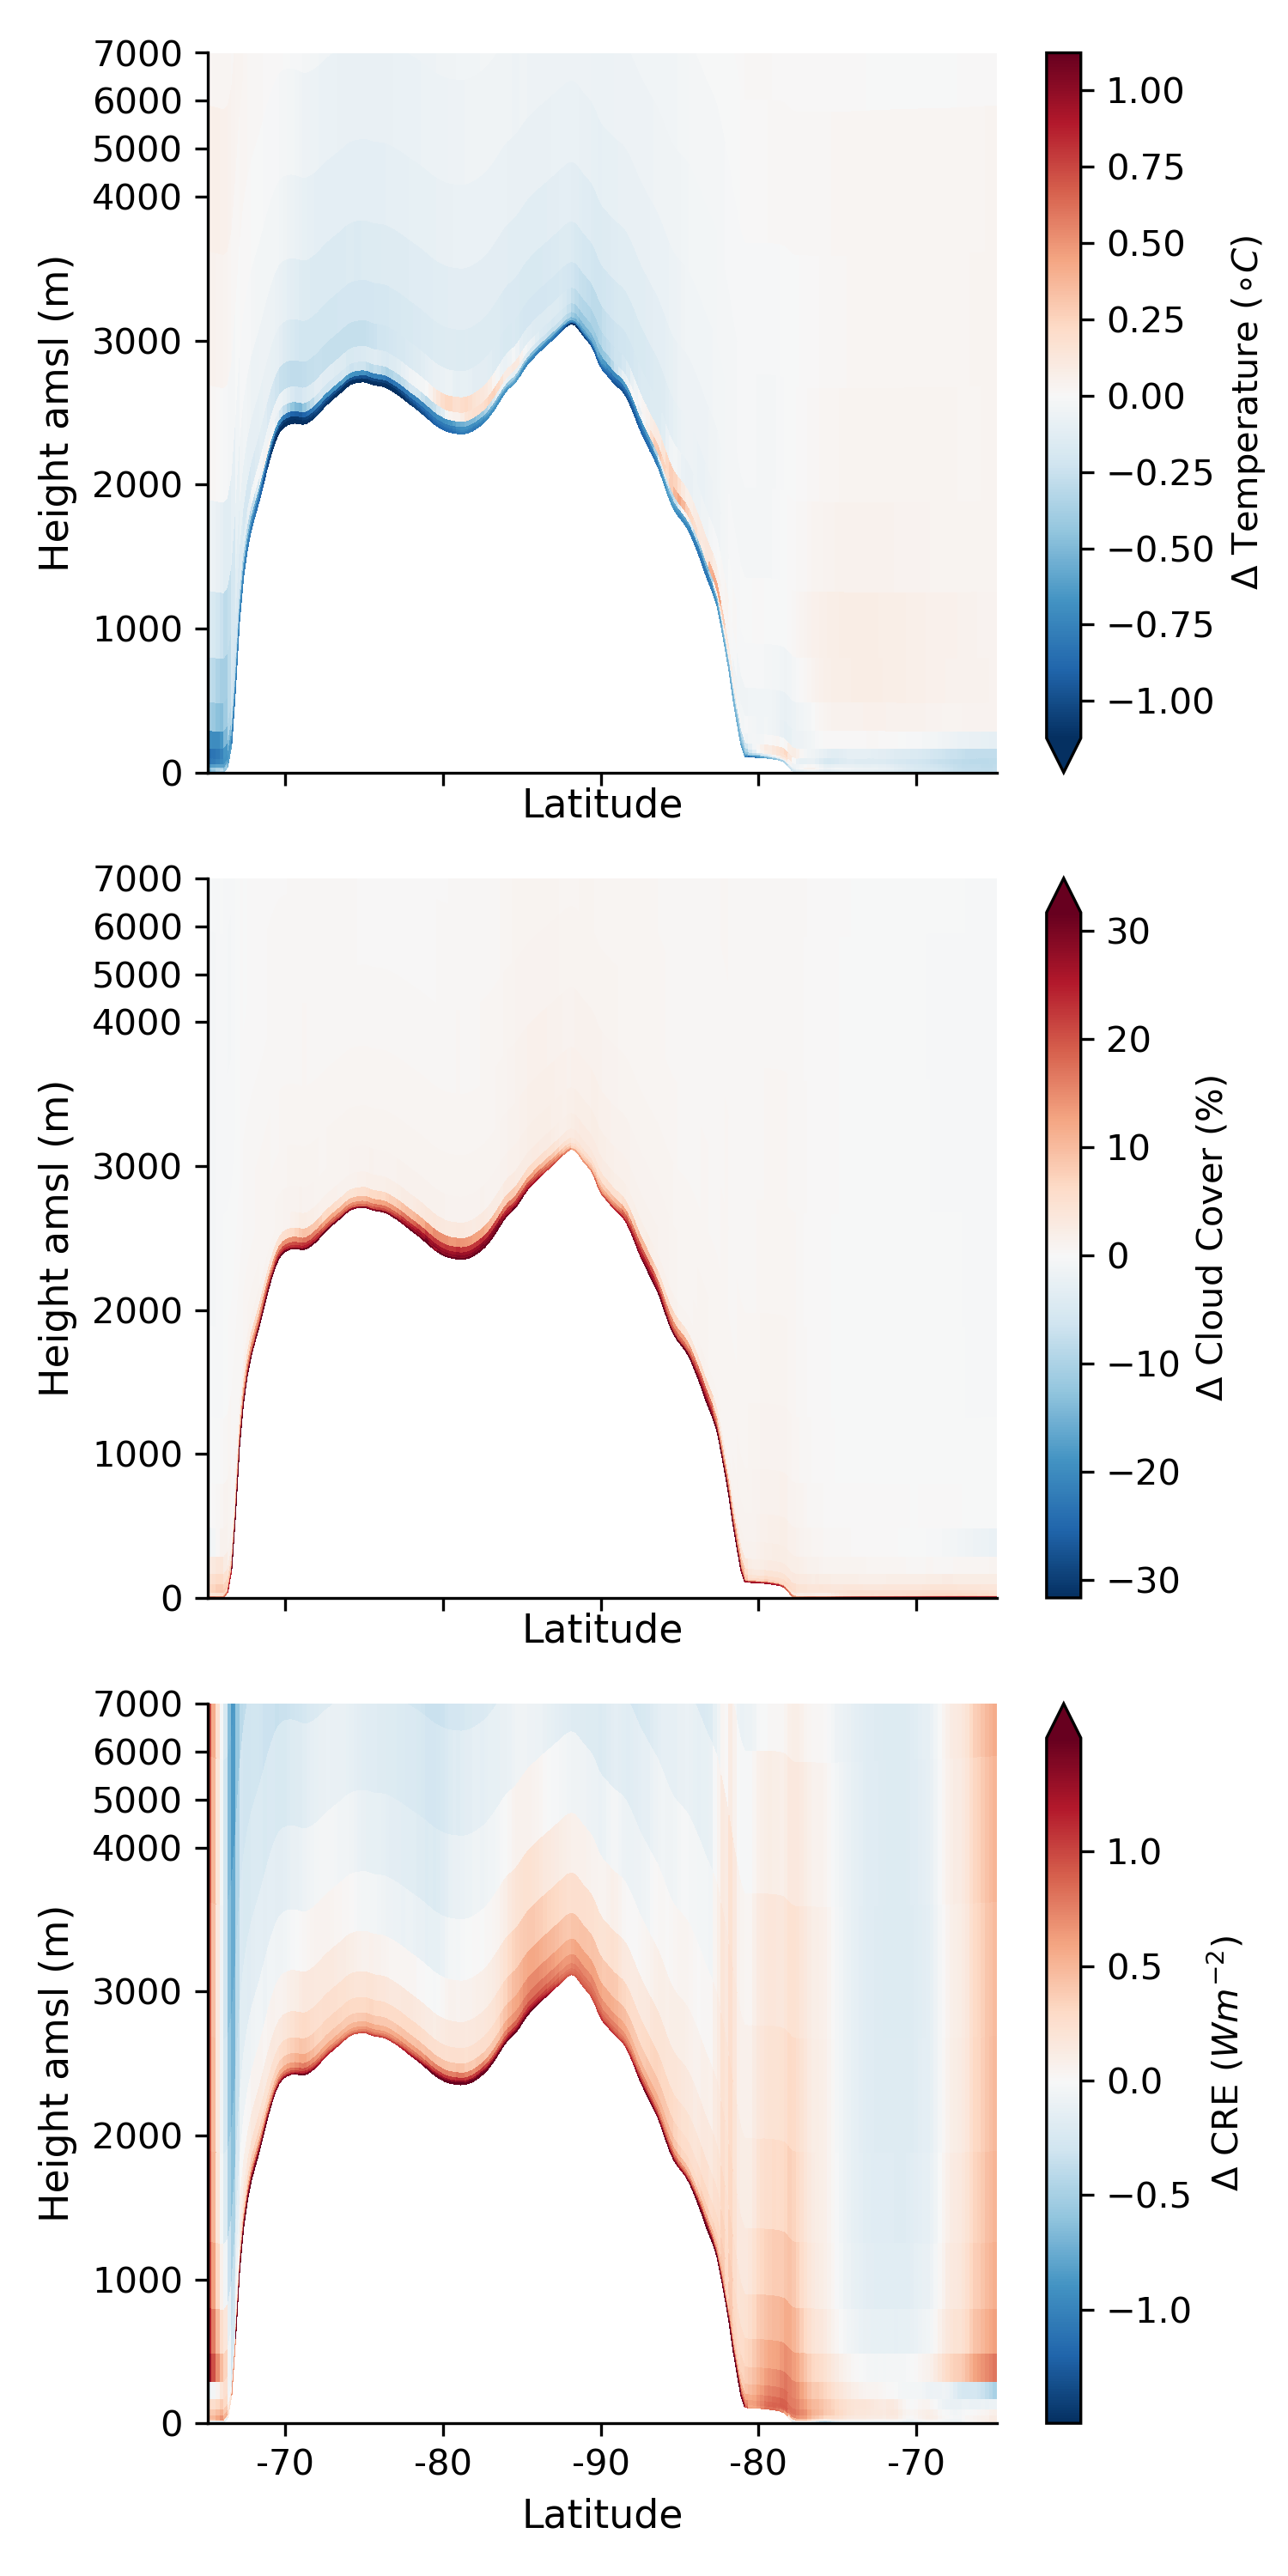
\includegraphics[scale=0.7,center]{cross_section_lt.png}
	\caption{\textbf{Difference in temperature and cloud properties between MAR with and without blowing snow.} A) Cross-section of temperature differences between MAR with blowing snow turned on, and MAR without blowing snow (positive means MARbs is warmer), along the path shown in \textbf{MISSING FIGURE XX}. B) Same as panel A), but showing the difference in cloud cover (in \%) between the two simulations. C) Same as panel A) and B), but for the difference in the cloud radiative effect ($Wm^{-2}$). }
	\label{fig:Test}
\end{figure}

In the boundary layer, accounting for drifting snow also increases cloud formation over the Antarctic continent (Fig.\ref{fig:Test}B). Our results show that the strongest increase in 2000-2019 average cloud cover over the interior plateau strongly overlap with the changes in temperature seen in Figure \ref{fig:Test}A. In elevations above 2000 m above mean sea level the lowermost 500 m of the atmosphere show an increase of \textbf{XX $\pm$ XX\%} in cloud cover. However, there are three overlapping mechanisms that can explain the greater cloud amount over the Antarctica, when accounting for blowing snow. 1) Blowing snow particles can act as additional nuclei on which ice can grow or help with ice growth through the Wegener-Bergeron-Findeisen process. Ice crystal number concentration can potentially multiplied through secondary ice processes \textbf{cite Sotiropoulou}. 2) The sublimation of airborne snow particles leads to a cooling of the surrounding air, while increasing the specific humidity, both bringing the environment closer to saturation (\textbf{Cite Amory saturation}). 3) Thick blowing snow layers themselves act as a cloud, due to their ability to interact with incoming solar radiation (i.e. a cloud optical depth > 0) and their influence on the atmospheric longwave emissivity (i.e. they increase the atmospheric longwave emissivity $\epsilon$). It is likely that in most cases these three processes can act simultaneously. Additionally, even state-of-the-art active satellite products like the \textbf{Cloudsat-Calipso XX}, have a vertical resolution of 240-480 m when looking at their cloud-related datasets. This limitation in vertical resolution renders it quite unlikely that blowing snow is detected as a cloud from remote sensing platforms, especially over highly-reflective surfaces.

Accounting for blowing snow also alters the cloud radiative effect (Fig.\ref{fig:Test} C). While we see the strongest effects again in the boundary layer, especially over the steeper margins the CRE is altered to elevations of up to 5000 m. This vertical influence on the CRE might be due to the fact that airborne blowing snow particles can be mixed to layers above the boundary layer in zones with stronger adiabatic mixing and turbulence, i.e. over the steeper slopes where the katabatic winds are the strongest. Subsequently, these additional ice crystals can influence the macrophysical cloud properties (IWP, LWP and COD), and therefore the CRE. Additionally, because of changes in the vertical temperature distribution and humidity due to blowing snow sublimation, also the effectiveness and temperature of the layers that emit the longwave radiation can be altered between the two simulations. 


\begin{figure}[H]
	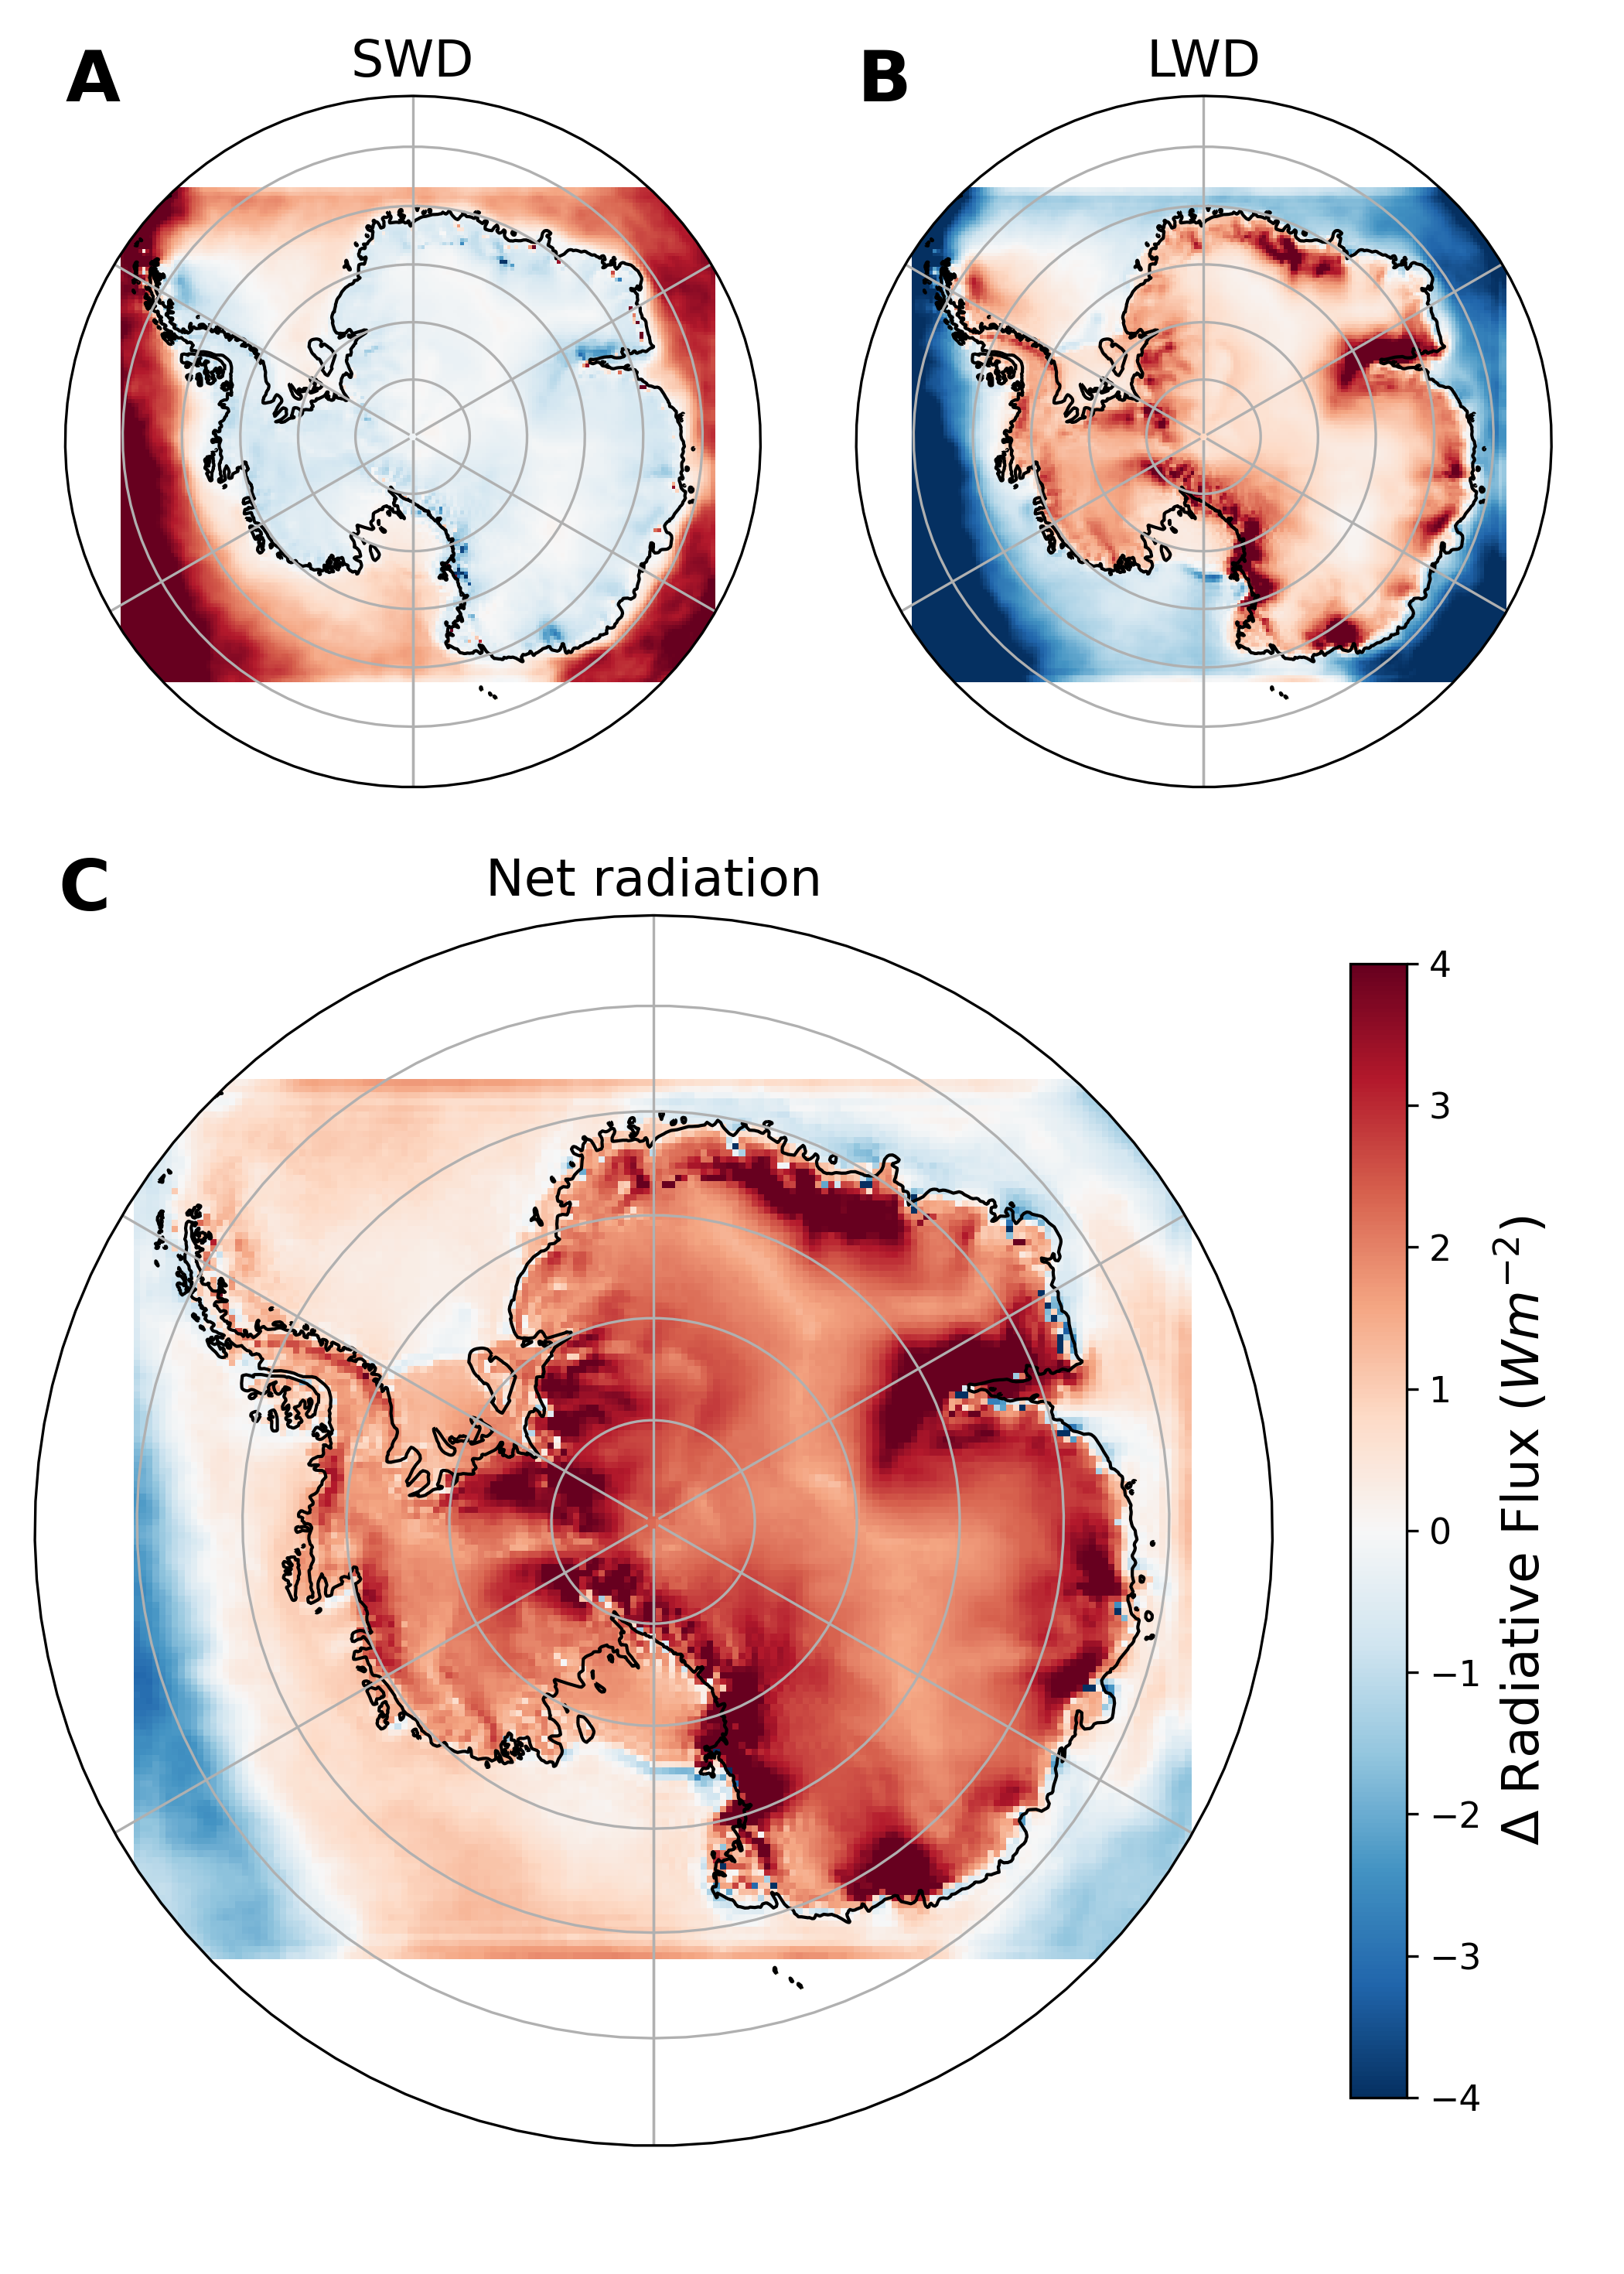
\includegraphics[scale=0.7,center]{SEB.png}
	\caption{\textbf{Difference in radiative components at the surface between MAR with and without blowing snow.} A) Difference in incoming shortwave radiation (SWD) at the surface in $Wm^{-2}$. Red color indicates a greater downwelling shortwave flux in MAR with active blowing snow parameterisation. B) Same A) but for the downwelling longwave flux at the surface. C) Same as A) and B), but for the difference in the net radiation at the surface ($R= SWD * (1 - \alpha) + LWD - LWU$).}
	\label{fig:SEB}
\end{figure}

To explore how the macrophysical cloud properties in MAR with snow differ from the base simulation without blowing snow, we show the spatial difference in cloud cover, cloud optical depth, liquid- and ice water path in Fig.\ref{fig:micro} A-D. Overall, our results show a clear signal of increased cloud cover over most of Antarctica (\textbf{AIS: XX $\pm$ XX, Ocean: XX $\pm$ XX}). Only over parts of the Souther Ocean do we see a small decrease in clouds (Fig.\ref{fig:micro}A). Over most of Antarctica our results indicate no changes in cloud optical depth (Fig.\ref{fig:micro}B). Interestingly, over the Southern Ocean and near the Antarctic peninsula we see areas with a strong COD increase (maximum \textbf{+XX}) and strong decreases (minimum \textbf{-XX}). This strong decrease in COD over open ocean waters is mainly a result of a decrease in LWP (Fig.\ref{fig:micro}C), in addition to a decrease in IWP (Fig.\ref{fig:micro}D). This decrease in COD, CC, LWP and IWP over the open ocean could be due to a decrease in cloud lifetime because of extra ice crystal numbers due to blowing snow, potentially increasing the glaciation rate of clouds via the Wegener-Bergeron-Findeisen process (\textbf{cite Storelvmo2011, Gallee}) and subsequent increase in precipitation efficiency upstream of the Southern Ocean (\textbf{cite Storelvmo2011}).

Conversely, over the drier and colder interior of Antarctica, we see almost no changes in COD, nor in LWP, despite a significant increase in cloud cover (Fig.\ref{fig:micro}A-C). However, our results suggest a widespread increase in cloud ice water path (Fig.\ref{fig:micro}D), with a mean over the AIS of \textbf{+XX}. Here, additional airborne particles likely increase the rate of new ice growth due to the Wegener-Bergeron-Findeisen process, which states that ice particles grow at the expense of liquid cloud condensate (\textbf{CITE WBF}). In our simulations this process seems to be most efficient over the steeper margins of Antarctica, where 1) snow mass transport increases with stronger katabatic winds, where 2) turbulence mixes snow and ice to higher elevations and where 3) the chances of mixed-phase clouds increases due to an increase in oceanic influence and higher temperatures than over the interior Antarctic plateau. Additionally, new ice particles can also in MAR due to higher relative humidity of the advected air via the gas phase or via heterogeneous and homogeneous freezing (\textbf{cite Gallee}). Note however, that the MAR cloud microphysics scheme currently does not account for secondary ice production, where one single ice crystal can turn into multiple ice crystals via collision breakup, drop shattering and rime splintering (\textbf{cite Sotiropoulou, Gallee, Storelvmo2011}). However, especially rime splintering and drop shattering need liquid to be present and are most efficient in temperatures above what we observe over Antarctica (\textbf{Sotiroupoulou}). Therefore, we don't think that the missing drop shattering and rime splintering processes are a major source of uncertainty in our simulations, however, collision breakup in blowing snow clouds could be an important missing multiplier of ice crystal number concentration in our simulations.


\begin{figure}[H]
	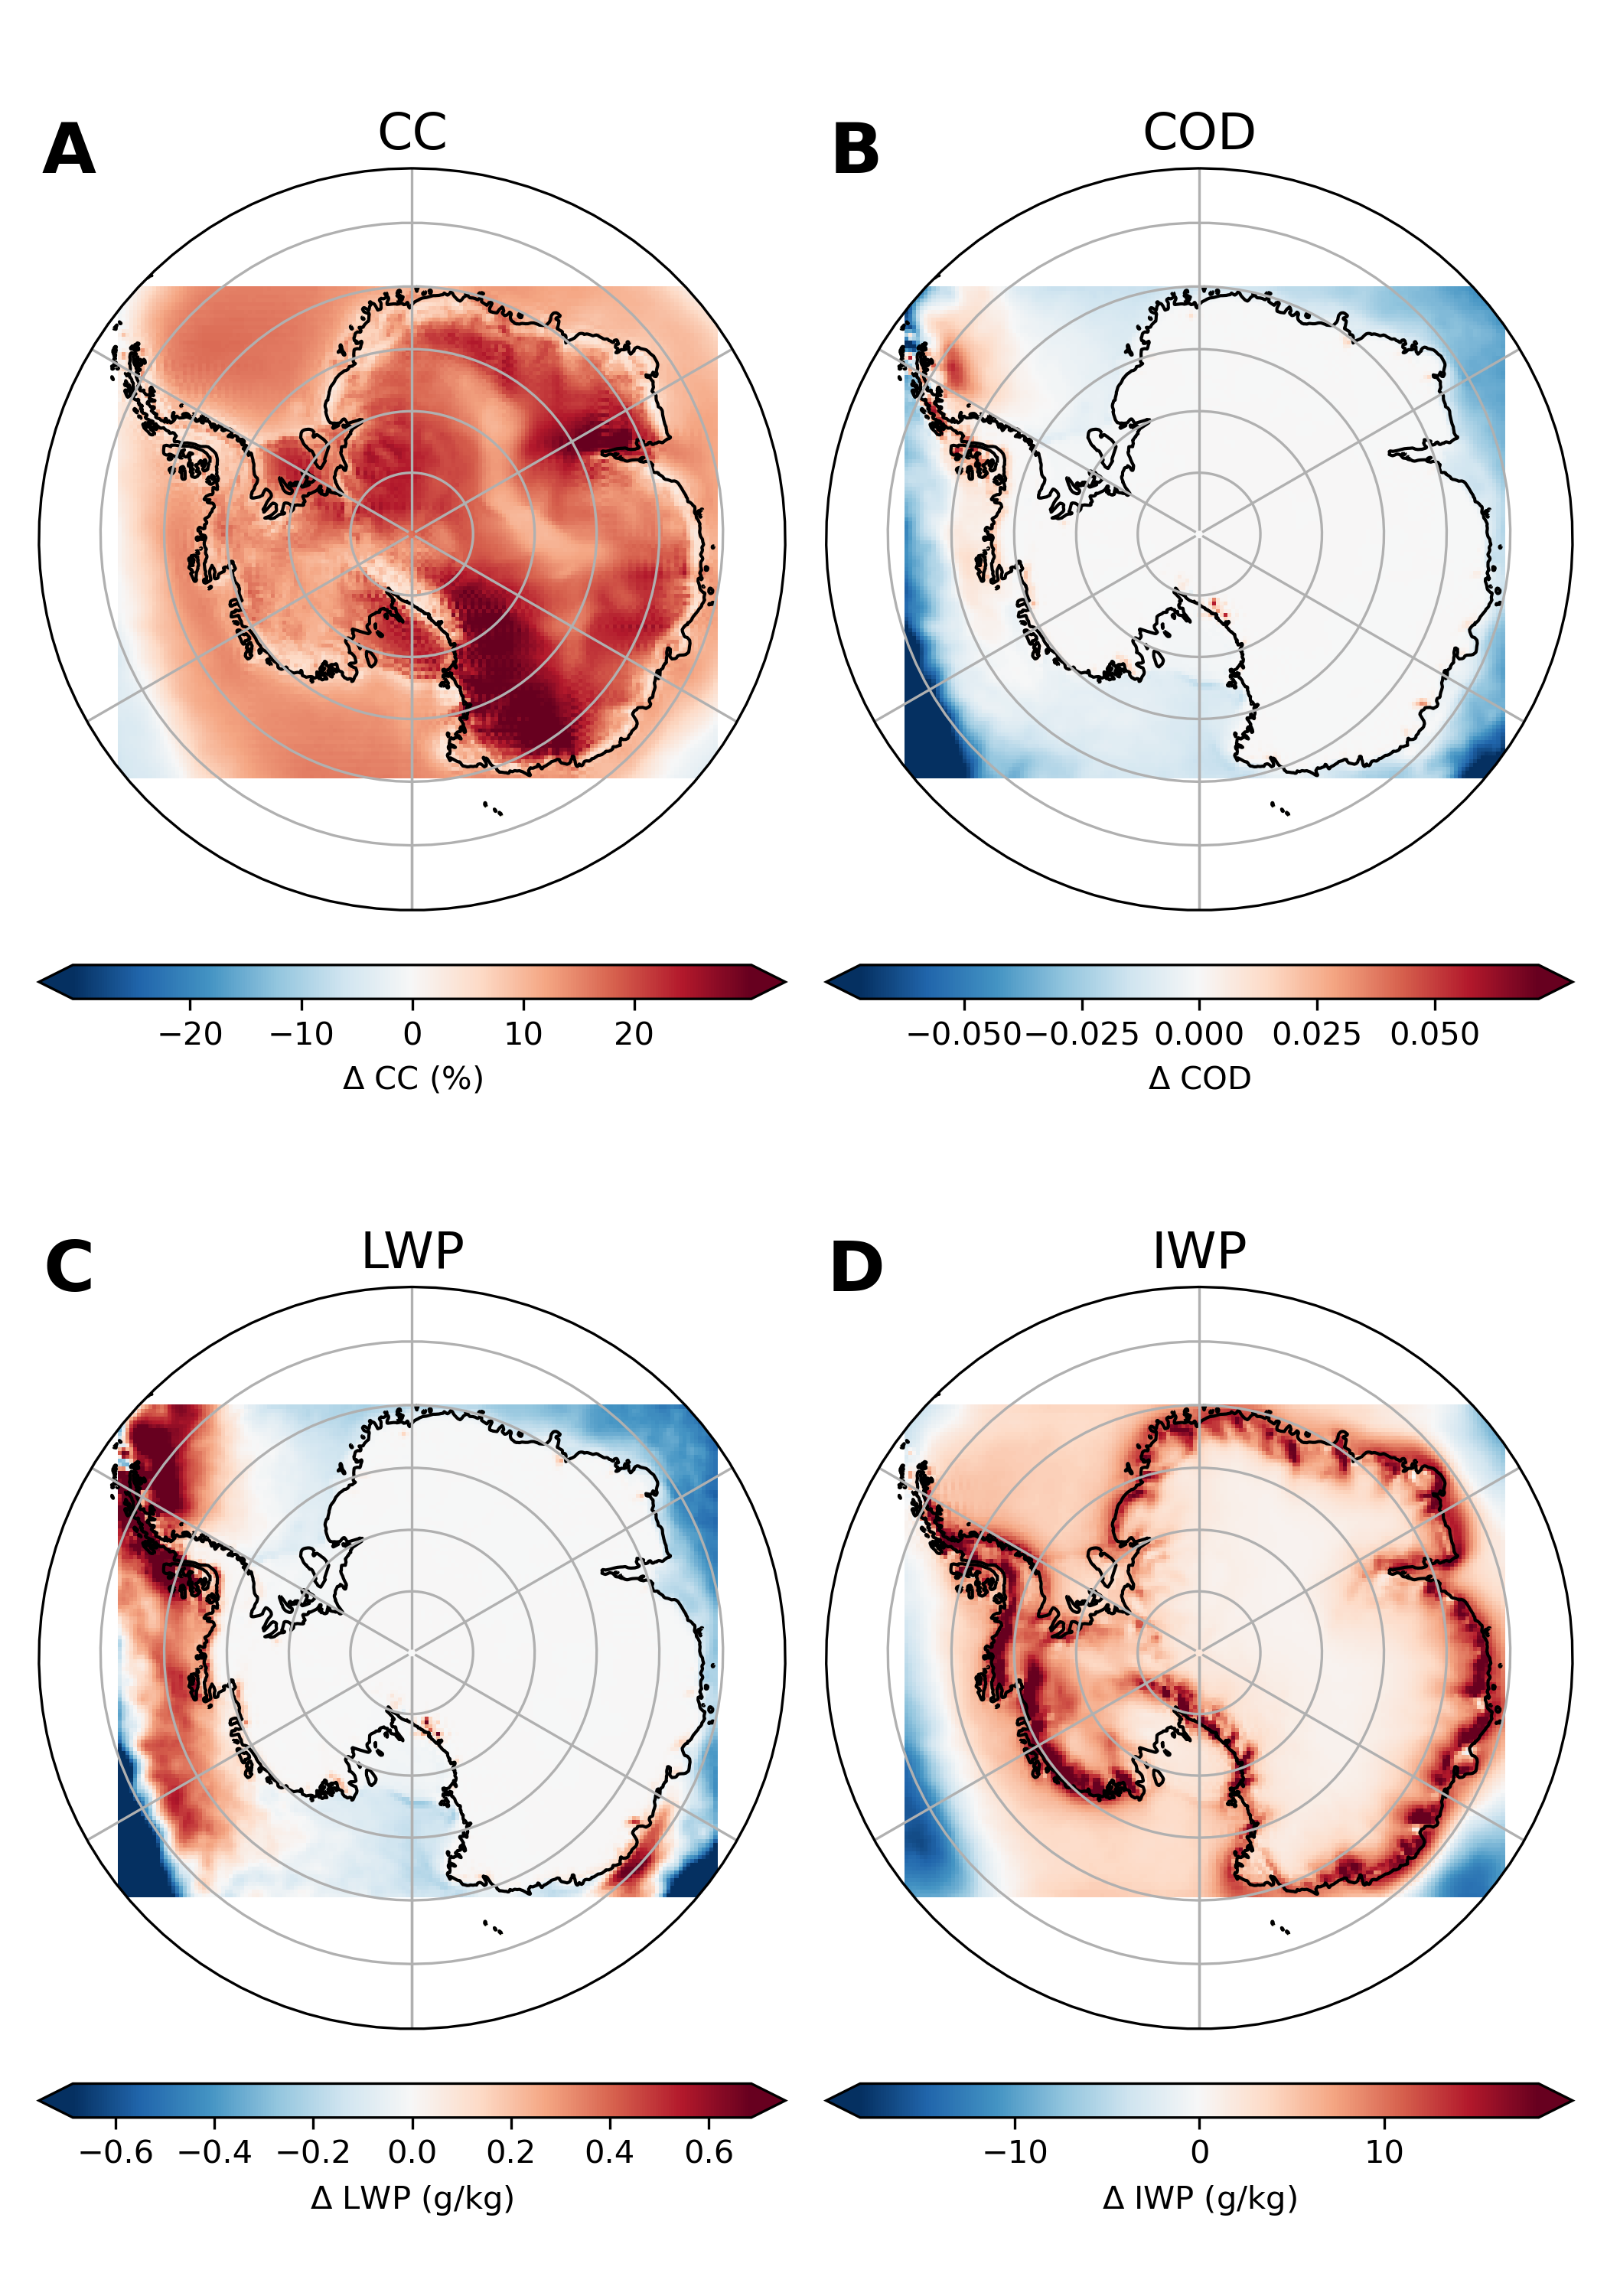
\includegraphics[scale=0.7,center]{microphysics.png}
	\caption{\textbf{Difference in cloud properties between MAR with and without blowing snow.} A) Difference in cloud cover (\%) between the two MAR simulations. Red colors indicate a greater cloud cover percentage in MAR with active blowing snow parameterisation. B) Same as A) but for the difference in cloud optical depth (COD, unitless) between the two MAR simulations. C) Same as A) but for the difference in liquid water path(LWP, g/kg). D) Same as A) but for the difference in ice water path (IWP, g/kg).}
	\label{fig:micro}
\end{figure}

\section*{Discussion}



%\nolinenumbers
\cleardoublepage
\printbibliography[title={Main References}]
%\printbibliography[keyword=main, title={Main References}]
%\end{refsection}

%\begin{refsection}
\baselineskip24pt
%\linenumbers
\section*{Materials and Methods}

\subsection*{MAR}

%
\subsection*{MODIS}

\subsection*{AVHRR}

\subsection*{ERA5}


\subsection*{Modèle Atmosphérique Régional (MAR)}
For the downscaling of coarse-resolution CMIP5 and CMIP6 data we used the Modèle Atmosphérique Régional (MAR), an open-source and widely used polar regional climate model
\cite{Fettweis2007,Fettweis2013,Fettweis2017,Gallee1994,Gallee1995,Hofer2017,Hofer2019,Kittel2018, Delhasse2018,Lang2015, Agosta2019}. MAR consists of a hydrostatic dynamical core which solves the primitive equation set \cite{Gallee1994,Gallee1995}. A full description of the model setup, the underlying physical parameterizations and evaluation of MAR for polar climates are described in \cite{Gallee1994,Gallee1995,Fettweis2007,Fettweis2017,Hofer2017,Hofer2019,Kittel2018,Agosta2019}. In this study we used the MARv3.9.6 version, evaluated in \textcite{Delhasse2019}, and the source code of MAR for the reproduction of this study is available via the MAR hompeage at \textbf{http://mar.cnrs.fr}.

Within MAR, the snow and ice properties at the ice sheet-atmosphere interface are calculated in the Soil Ice Vegetation Atmosphere Transfer module (SISVAT) \cite{Gallee1994}. This module calculates the main snowpack based on the snow module CROCUS \cite{Gallee2001,Vionnet2012}, but also handles the mass and energy exchange between the atmosphere (e.g. radiation, precipitation, temperature) and the bare-ice surfaces, the snowpack and the Arctic tundra that surrounds the GrIS \cite{Gallee1994,Fettweis2007}.

For the 6 CMIP5 and 5 CMIP6 future projections we downscaled we prescribed the boundary conditions in exactly the same manner and also used the MAR version and setup throughout. Overall, MAR was forced at its lateral boundaries (pressure, wind speed, temperature, specific humidity), at the top of the stratosphere (temperature, wind speed) and at the ocean surface (sea ice concentration, sea surface temperature) every 6 hours using GCM and ERA-Interim reanalysis fields \cite{Agosta2019,Kittel2018,Fettweis2007,Fettweis2013}. We ran MAR at a spatial resolution of 15 km x 15 km on a polar stereographic projection, which represents a significant increase in resolution compared to previous GrIS regional climate projections with MAR in \textcite{Fettweis2013}, and which was used in the IPCC AR5 \cite{IPCC2014}. The MAR setup used in this study has been thoroughly compared to observations from weather stations, observed radiative fluxes, satellite cloud cover, satellite albedo and melt extent, ablation and SMB in-situ measurements \cite{Tedesco2019,Fettweis2007,Fettweis2017,Hofer2017,Delhasse2019}. 





\nolinenumbers
\cleardoublepage
\printbibliography[keyword=methods, title={Methods References}]
%\end{refsection}
%\section*{Supplementary material}
%\begin{figure}[H]
%	\includegraphics[scale=0.90,center]{SMB.png}
%	\caption*{} 
%	\label{fig:S1}
%\end{figure}



\section*{Acknowledgments}
This project has received funding from the European Research Council (ERC) under the European Union’s Horizon 2020 research and innovation programme (Grant agreement No. 758005). Computational resources have been provided by the Consortium des Equipements de Calcul Intensif (CECI), funded by the Fonds de la Recherche Scientifique de Belgique (F.R.S.-FNRS) under grant no. 2.5020.11 and the Tier-1 supercomputer (Zenobe) of the Fédération Wallonie Bruxelles infrastructure funded by the Walloon Region under the grant agreement no. 1117545. This work was also supported by the Fonds de la Recherche Scientifique (FNRS) and the Fonds Wetenschappelijk Onderzoek-Vlaanderen (FWO) under the EOS Project n° O0100718F. 
We thank Katherine Thayer-Calder and William Lipscomb for providing 6-hourly output data from CESM2.

\section*{Author contributions}

S.H., C.K., C.A., X.F., C.L. and A.T. designed the study. S.H. analyzed the data and wrote the manuscript. C.L. provided the analysis for the supplementary material. X.F. did the MAR simulations. All authors discussed the final version of manuscript.

\section*{Competing interests}
The authors declare that they have no competing interests.

\section*{Code and data availability}

%The monthly means used in this study, from 1980-2100 of all three MAR RCP 8.5 simulations are available via ftp://ftp.climato.be/fettweis/MARv3.9/Greenland/. In case daily outputs are required, these can be requested from Xavier Fettweis (xavier.fettweis@uliege.be) and Stefan Hofer (s.hofer@bristol.ac.uk).
%
All the code used for the analysis in this study is available upon request from the corresponding author (stefan.hofer@geo.uio.no). All the MAR model results are available for download on ftp://ftp.climato.be/fettweis/MARv3.9/ISMIP6/GrIS/ in the framework of the ISMIP6 exercise (https://tc.copernicus.org/articles/14/2331/2020/).






\end{document}